\chapter{Client interaction}
\label{clients}

\begin{figure}
\centering
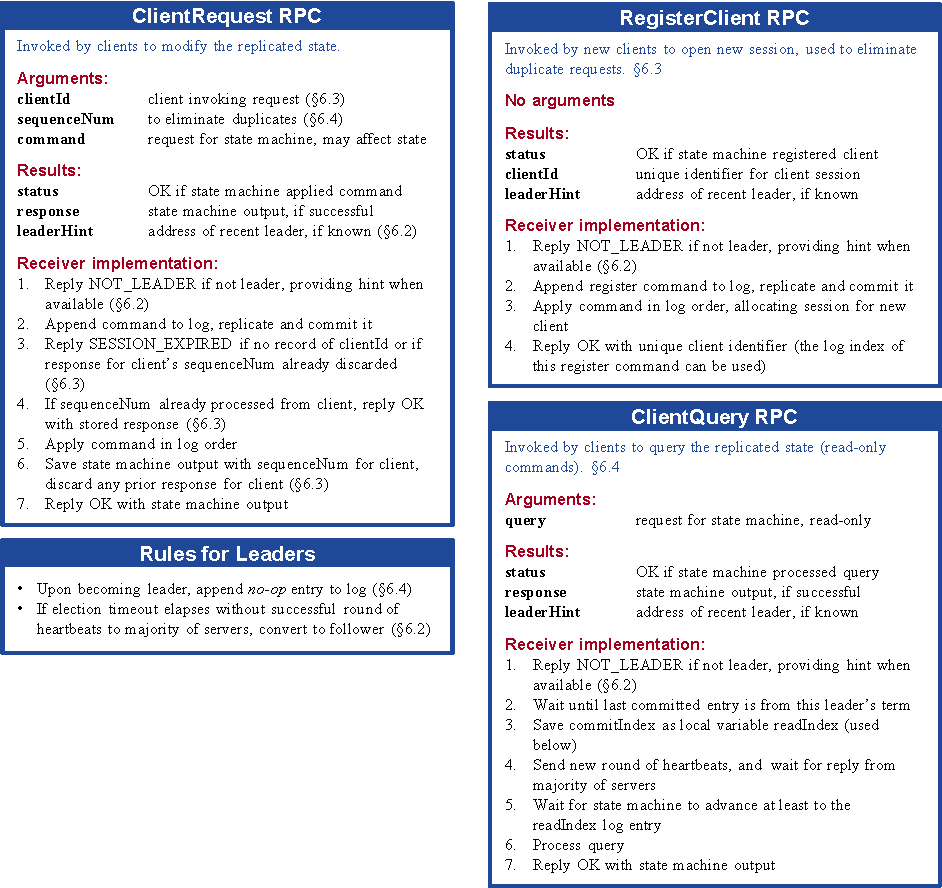
\includegraphics[scale=0.95]{clients/cheatsheet}
\vcaption[summary of RPCs]{
Clients invoke the ClientRequest RPC to modify the replicated state;
they
invoke the ClientQuery RPC to query the replicated state. New clients
receive their client identifier using a RegisterClient RPC, which helps
identify when session information needed for linearizability has been discarded.
In the figure, servers that are not leaders
redirect clients to the leader, and read-only requests are serviced
without relying on clocks for linearizability (the text presents
alternatives).
Section numbers such as \S\ref{clients:linearizability} indicate where
particular features are discussed.
}
\label{fig:clients:cheatsheet}
\end{figure}

This chapter describes several issues in how clients interact with a
Raft-based replicated state machine:
\begin{compactitem}
\item Section~\ref{clients:findcluster} describes how clients find the
cluster, even when its set of members can change over time;
\item Section~\ref{clients:findleader} describes how clients' requests
are routed to the cluster leader for processing;
\item Section~\ref{clients:linearizability} describes how Raft provides
linearizable consistency~\cite{Herlihy:1990}; and
\item Section~\ref{clients:readonly} describes how Raft can process
read-only queries more efficiently.
\end{compactitem}
Figure~\ref{fig:clients:cheatsheet} shows the RPCs that clients use to
interact with the replicated state machine; the elements of these RPCs are
discussed throughout the chapter.
These issues apply to all consensus-based systems, and
Raft's solutions are similar to other systems.

This chapter assumes that the Raft-based replicated state machine
is exposed to clients directly as a network service. Raft can
alternatively be
integrated directly into a client application. In this case, some issues
in client interaction may be pushed up a level to network clients of the
embedding application. For example, network clients of the embedding
application would have a similar problem in finding the application's cluster
as clients of a Raft network service have in finding the Raft cluster.

\section{Finding the cluster}
\label{clients:findcluster}

When Raft is exposed as a network service,
clients must locate the cluster in order to interact with the replicated
state machine.
For clusters with fixed membership, this is straightforward; for
example, the network addresses of the servers can be stored statically
in a configuration file. However, finding the cluster when its set of
servers can change over time (as described in Chapter~\ref{membership})
is a bigger challenge. There are two general approaches:
%
\begin{enumerate}
%
\item Clients can use network broadcast or multicast to find all cluster
servers. However, this will only work in particular environments that
support these features.
%
\item Clients can discover cluster servers via an external directory
service, such
as DNS, that is accessible at a well-known location. The list of servers
in this external system need not be consistent, but it should be inclusive:
clients should always be able to find all of the cluster servers, but
including a few additional servers that are not currently members of the
cluster is harmless. Thus, during cluster membership changes, the
external directory
of servers should be updated before the membership change to include any
servers soon to be added to the cluster, then updated again after the
membership change is complete to remove any servers that are no longer
part of the cluster.
%
\end{enumerate}
%
%
LogCabin clients currently use DNS to find the cluster. LogCabin does not
currently update DNS records automatically before and after membership
changes (this is left to administrative scripts).

\section{Routing requests to the leader}
\label{clients:findleader}

Client requests in Raft are processed through the leader, so clients
need a way to find the leader.
When a client
first starts up, it connects to a randomly chosen server. If the
client's first choice is not the leader, that server rejects the
request. In this case, a very simple approach is for the client to try
again with another randomly chosen server until it finds the leader.
If clients choose servers randomly
without replacement, this na\"ive approach is expected to find the
leader of an $n$-server cluster after $\dfrac{n+1}{2}$ attempts,
which may be fast enough for small clusters.

Routing requests to the leader can also be made faster with simple
optimizations. Servers usually know the address of the current cluster
leader, since AppendEntries requests include the leader's identity.
When a server that is not leader receives a request from a
client, it can do one of two things:
%
\begin{enumerate}
%
\item The first option, which we recommend and which LogCabin
implements, is for the server to reject
the request and return to the client the address of the leader, if
known. This allows the client to reconnect to the leader directly,
so future requests can proceed at full speed. It also takes very
little additional code to implement, since clients already need to
reconnect to a different server in the event of a leader failure.
%
\item
Alternatively, the server can proxy the client's request to the
leader.
This may be simpler in some cases. For example, if a client connects
to any server for read requests (see Section~\ref{clients:readonly}),
then proxying the client's write requests would save the client from
having to manage a distinct connection to the leader used only for writes.
%
\end{enumerate}

Raft must also prevent stale leadership information from delaying client
requests indefinitely. Leadership information can become stale all
across the system, in leaders, followers, and clients:
%
\begin{itemize}
%
\item \textbf{Leaders:} A server might be in the leader state, but if it
isn't the current leader, it could be needlessly delaying client
requests. For example, suppose a leader is partitioned from the rest of
the cluster, but it can still communicate with a particular client.
Without additional mechanism, it could delay a request from that client
forever, being unable to replicate a log entry to any other servers.
Meanwhile, there might be another leader of a newer term that
is able to communicate with a majority of the cluster and would be able
to commit the client's request. Thus, a leader in Raft steps down if an
election timeout elapses without a successful round of heartbeats to a
majority of its cluster; this allows clients to retry their requests
with another server.
%
\item \textbf{Followers:} Followers keep track of the leader's identity
so that they can redirect or proxy clients. They must discard this
information when starting a new election or when the term changes.
Otherwise, they might needlessly delay clients (for example, it would be
possible for two servers to redirect to each other, placing clients in
an infinite loop).
%
\item \textbf{Clients:} If a client loses its connection to the leader
(or any particular server), it should simply retry with a random server.
Insisting on being able to contact the last known leader would result in
unnecessary delays if that server failed.
%
\end{itemize}

\section{Implementing linearizable semantics}
\label{clients:linearizability}


\begin{figure}
\centering
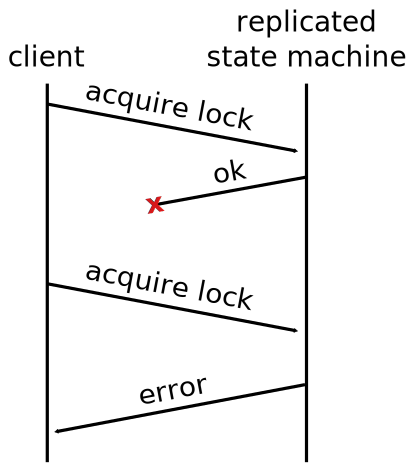
\includegraphics[scale=0.45]{clients/retrydup}
\vcaption[example of incorrect results for duplicated command]{
An example of an incorrect results that can arise from
duplicated commands. A client submits a command to a replicated state
machine to acquire a lock. The client's first command acquires the lock,
but the client never receives the acknowledgment. When the client
retries the request, it finds that the lock is already taken.
}
\label{fig:clients:retrydup}
\end{figure}

As described so far, Raft provides at-least-once semantics for clients;
the replicated state machine may apply a command multiple times. For
example, suppose a client submits a command to a leader and the leader
appends the command to its log and commits the log entry, but then it
crashes before responding to the client. Since the client receives no
acknowledgment, it resubmits the command to the new leader, which in
turn appends the command as a new entry in its log and also commits this
new entry. Although the client intended for the command to be executed
once, it is executed twice. Commands can also be applied multiple times
even without the client's involvement if the network may duplicate the
client's requests.

This issue is not unique to Raft; it occurs in most stateful distributed
systems. However, these at-least-once semantics are particularly
unsuitable for a consensus-based system, where clients typically need
stronger guarantees. Problems from duplicated commands can manifest in
subtle ways that are difficult for clients to recover from. These
problems cause either incorrect results, incorrect states, or both.
Figure~\ref{fig:clients:retrydup} shows an example of an incorrect
result: a state machine is providing a lock, and
a client finds it is unable to acquire the lock because its
original request---for which it received no acknowledgment---has
already acquired the lock. An example of an incorrect state would be an
increment operation, where the client intends for a value to increment
by one but it instead increments by two or more. Network-level
reordering and concurrent clients can lead to even more surprising
results.

Our goal in Raft is to implement linearizable semantics~\cite{Herlihy:1990}, which avoid
these classes of problems. In linearizability, each operation appears to
execute instantaneously, exactly once, at some point between its
invocation and its response. This is a strong form of consistency that
is simple for clients to reason about, and it disallows commands being
processed multiple times.

To achieve linearizability in Raft, servers must filter out duplicate
requests. The basic idea is that servers save the results of
client operations and use them to skip executing the same request
multiple times.
To implement this, each client is given a unique
identifier, and clients assign unique serial numbers to every command.
Each server's state machine maintains a \emph{session} for each client.
The session tracks the latest serial number processed for the
client, along with the associated response. If a server receives a command
whose serial number has already been executed, it responds immediately
without re-executing the request.

Given this filtering of duplicate requests, Raft
provides linearizability. The Raft log provides a serial order in which
commands are applied on every server. Commands take effect
instantaneously and exactly once according to their first appearance in
the Raft log, since any subsequent appearances are filtered out by the
state machines as described above.

This approach also generalizes to allow concurrent requests from a
single client. Instead of the client's session tracking just the
client's latest sequence number and response, it includes a set of
sequence number and response pairs. With each request, the client
includes the lowest sequence number for which it has not yet received a
response, and the state machine then discards all responses for lower
sequence numbers.



Unfortunately, sessions cannot be kept forever, as space is
limited. The servers must eventually decide to expire a client's
session, but this creates two problems: how can servers agree on when to
expire a client's session, and how can they deal with an active client
whose session was unfortunately expired too soon?

Servers must agree on when to expire a client's session; otherwise,
servers' state machines could diverge from each other. For example,
suppose one server expired the session for a particular client, then
re-applied many of that client's duplicated commands; meanwhile, the
other servers kept the session alive and did not apply the duplicates.
The replicated state machine would become inconsistent. To avoid such
problems,
session expiry must be deterministic, just as normal state machine
operations must be. One option is to set an upper bound on the number
of sessions and remove entries using an LRU (least recently used)
policy. Another option is to expire sessions based on an agreed upon
time source. In LogCabin, the leader augments each command that it
appends to the Raft log with its current time. Servers reach
agreement on this time as part of committing the log entry; then, the
state machines deterministically use this time input to expire inactive
sessions. Live clients issue keep-alive requests during
periods of inactivity,
which are also augmented with the leader's timestamp and committed to
the Raft log, in order to maintain their sessions.

The second issue is how to deal with a client that continues to operate
after its session was expired. We expect this to be an exceptional
situation; there is always some risk of it, however, since there is
generally no way to know when clients have exited. One option would be
to allocate a new session for a client any time there is no record of
it, but this would risk duplicate execution of commands that were
executed before the client's previous session was expired.
To provide stricter guarantees,
servers need to distinguish a new client from a client whose session was
expired. When a client first starts up, it can register itself with
the cluster using the RegisterClient RPC. This
allocates the new client's session and returns the client its
identifier, which the client includes with all subsequent commands. If a
state machine encounters a command with no record of the session, it
does not process the command and instead returns an error to the client.
LogCabin currently crashes the client in this case (most clients
probably wouldn't handle session expiration errors gracefully and
correctly, but systems must typically already handle clients crashing).

\section{Processing read-only queries more efficiently}
\label{clients:readonly}

Read-only client commands only query the replicated state machine; they
do not change it. Thus, it is natural to ask whether these queries can
bypass the Raft log, whose purpose is to replicate changes to the
servers' state machines in the same order. Bypassing the log offers an
attractive performance advantage: read-only queries are common in many
applications, and the synchronous disk writes needed to append entries
to the log are time-consuming.

However, without additional precautions, bypassing the log could lead to
stale results for read-only queries.
For example, a leader might be partitioned from the rest of the
cluster, and the rest of the cluster might have elected a new leader and
committed new entries to the Raft log. If the partitioned leader
responded to a read-only query without consulting the other servers,
it would return stale results, which are not linearizable.
Linearizability requires the results of a read to reflect a state of the
system sometime after the read was initiated; each read must at least
return the results of the latest committed write.
(A system that allowed stale reads would only provide
serializability, which is a weaker form of consistency.)
Problems due to stale reads have already been discovered in two
third-party Raft implementations~\cite{Kingsbury:etcdconsul},
so this issue deserves careful attention.

Fortunately, it is possible to bypass the Raft log for read-only queries
and still preserve linearizability. To do so, the leader takes the
following steps:
%
%
\begin{enumerate}
%
\item If the leader has not yet marked an entry from its current term
committed, it waits until it has done so. The Leader Completeness
Property guarantees that a leader has all committed entries, but at the
start of its term, it may not know which those are. To find out, it
needs to commit an entry from its term. Raft handles this by having each
leader commit a blank \emph{no-op} entry into the log at the start of
its term. As soon as this no-op entry is committed, the leader's commit
index will be at least as large as any other servers' during its term.
%
\item The leader saves its current commit index in a local
variable
\emph{readIndex}. This will be used as a lower bound for the version
of the state that the query operates against.
%
\item The leader needs to make sure it hasn't been 
superseded by a newer leader of which it is unaware.
It issues a
new round of heartbeats and waits for their acknowledgments from a
majority of the cluster. Once these acknowledgments are received, the
leader knows that there could not have existed a leader for a greater
term at the moment it sent the heartbeats. Thus, the readIndex was, at
the time, the largest commit index ever seen by any server in the
cluster.
%
\item The leader waits for its state machine to advance at least as far
as the readIndex; this is current enough to satisfy
linearizability.
%
\item Finally, the leader issues the query against its state machine and
replies to the client with the results.
%
\end{enumerate}

This approach is more efficient than committing read-only queries as new
entries in the log, since it avoids synchronous disk writes. To improve
efficiency further, the leader can amortize the cost of confirming its
leadership: it can use a single round of heartbeats for any number of
read-only queries that it has accumulated.

Followers could also help offload the processing of read-only queries.
This would improve the system's read throughput, and it would also
divert load away from the leader, allowing the leader to process more
read-write requests. However, these reads would also run the risk of
returning stale data without additional precautions. For example, a
partitioned follower might not receive any new log entries from the
leader for long periods of time, or even if a follower received a
heartbeat from a leader, that leader might itself be deposed and not yet
know it. To serve reads safely, the follower could issue a request to
the leader that just asked for a current readIndex (the leader would
execute steps 1--3 above); the follower could then execute steps 4 and 5
on its own state machine for any number of accumulated read-only
queries.

LogCabin implements the above algorithm on leaders, and it amortizes the
cost of the heartbeats across multiple read-only queries under high
load. Followers in LogCabin do not currently serve read-only requests.

\subsection{Using clocks to reduce messaging for read-only queries}



Up until now, the approach to read-only queries presented has provided
linearizability in an asynchronous model (where clocks, processors, and
messages can all operate at arbitrary speeds). This level of safety
requires communication to achieve: it requires a round of heartbeats to
half the cluster for each batch of read-only queries, which adds
latency to the queries.
The remainder of this section explores an alternative in which read-only
queries would avoid sending messages altogether by relying on clocks.
LogCabin does not currently implement this alternative, and we do not
recommend using it unless necessary to meet performance requirements.

\begin{figure}
\centering
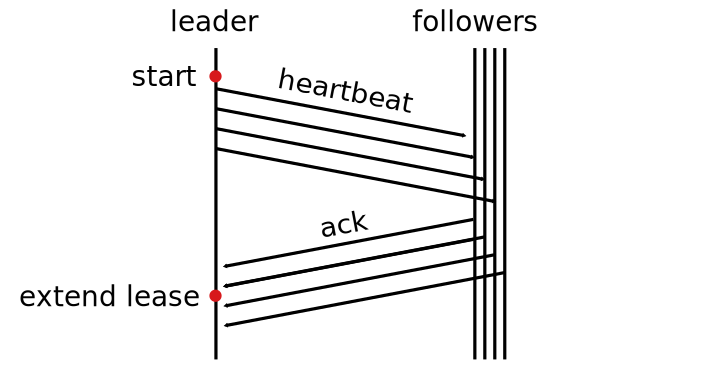
\includegraphics[scale=0.45]{clients/leases}
\vcaption[lease mechanism for read-only queries]{
To use clocks instead of messages for read-only queries,
the leader would use the normal heartbeat mechanism to maintain a lease.
Once the leader's heartbeats were acknowledged by a majority of the
cluster, it would extends its lease to $\textit{start} + \dfrac{\textit{election
timeout}}{\textit{clock drift bound}}$, since the followers
shouldn't time out before then.
While the leader held its lease, it would service read-only queries
without communication.
}
\label{fig:clients:leases}
\end{figure}

To use clocks instead of messages for read-only queries,
the normal heartbeat mechanism
would provide a form of lease~\cite{Gray:1989}.
Once the
leader's heartbeats were acknowledged by a majority of the cluster, the
leader would assume that no other server will become leader for about an
election timeout, and it could extend its lease accordingly (see
Figure~\ref{fig:clients:leases}). The leader would then reply to
read-only queries during that period without any additional
communication. (The leadership transfer mechanism presented in
Chapter~\ref{basicraft} allows the leader to be replaced early; a leader
would need to expire its lease before transferring leadership.)

The lease approach assumes a bound on clock drift across servers (over a
given time period, no server's clock increases more than this bound
times any other). Discovering and maintaining this bound might present
operational challenges (e.g., due to scheduling and garbage collection
pauses, virtual machine migrations, or clock rate adjustments for time
synchronization). If the assumptions are violated, the system could
return arbitrarily stale information.

Fortunately, a simple extension can improve the guarantee provided to
clients, so that even under asynchronous assumptions (even if clocks
were to misbehave), each client would see the replicated
state machine progress monotonically (sequential consistency).
For example, a client would not see the state as of log index $n$, then
change to a different server and see only the state as of log index $n-1$.
To implement this guarantee, servers would include the index
corresponding to the state machine state with each reply to clients.
Clients would track the latest index corresponding to results they had
seen, and they would provide this information to servers on each
request. If a server received a request for a client that had seen an
index greater than the server's last applied log index, it would not
service the request (yet).

\section{Conclusion}

This chapter discussed several issues in how clients interact with Raft.
The issues of providing linearizability and optimizing read-only queries
are particularly subtle in terms of correctness. Unfortunately, when the
consensus literature only addresses the communication between cluster
servers, it leaves these important issues out. We think this is a
mistake. A complete system must interact with clients correctly,
or the level of consistency provided by
the core consensus algorithm will go to waste. As we've already seen in
real Raft-based systems, client interaction can be a major source of
bugs, but we hope a better understanding of these issues can help prevent
future problems.

